%++++++++++++++++++++++++++++++++++++++++
% Don't modify this section unless you know what you're doing!
\documentclass[letterpaper,12pt]{article}
\usepackage{tabularx} % extra features for tabular environment
\usepackage{amsmath}  % improve math presentation
\usepackage{graphicx} % takes care of graphic including machinery
\usepackage[margin=1in,letterpaper]{geometry} % decreases margins
\usepackage{cite} % takes care of citations
\usepackage{indentfirst}
\usepackage[final]{hyperref} % adds hyper links inside the generated pdf file
\hypersetup{
	colorlinks=true,       % false: boxed links; true: colored links
	linkcolor=blue,        % color of internal links
	citecolor=blue,        % color of links to bibliography
	filecolor=magenta,     % color of file links
	urlcolor=blue         
}
%++++++++++++++++++++++++++++++++++++++++

% anything after % is a comment
%paragraph indentation
\setlength{\parindent}{2em} 

%paragraph spacing
\setlength{\parskip}{1em}

%Line spacing
\renewcommand{\baselinestretch}{1.5}

\usepackage{blindtext}
\begin{document}
\begin{titlepage}
	\centering
	
\includegraphics[width=0.40\textwidth]{usf.png}\par\vspace{0.1cm}
	{\scshape\LARGE MAD 4401: Numerical Analysis I \par}
	\vspace{1cm}
	{\scshape\Large Final Project\par}
	\vspace{1cm}
	{\huge\bfseries Approximating Pi\par}
	\vspace{1cm}
	{\Large\itshape Alexa Scott, Brennon Toomepuu, Rohit Vishen, Deanna Ramnarine, Kenya Quinones \par}
	\vfill
	

	\vfill

% Bottom of the page
	{\date{\textbf{Due Date:} December 3, 2019}\par}
\end{titlepage}




\pagebreak
\section{Abstract}

\indent The approximation of $\pi$ has been done throughout the history of mathematics. Pi's approximation is significant because it shows the differing accuracy of various numerical methods. The methods used for the purpose of this research project were Euler's method, Taylor's method, Simpson's Rule, Runge-Kutta method, and Adams Fourth Order Predictor-Corrector method. Our finding's showed that Simpson's Rule was the most accurate method as it approximated $\pi$ to twelve decimal places. The second most accurate method was Runge-Kutta approximating $\pi$ to ten decimal places. Taylor's and Adam's method tied for accuracy by approximating $\pi$ up to nine digits. Euler's method was the least accurate with an approximation up to six digits.    



\section{Introduction}

The number $\pi$, also known as Archimedes' constant, has been around for centuries, yet its precise value has yet to be fully determined. As its alternative name would suggest, $\pi$ was first calculated by Archimedes as the ratio between a circle’s circumference and its diameter, hence the common definition of $\pi$ we typically see; $\pi = C/d$ \cite{Gorleau03}. Since this discovery, $\pi$ has been used for various tasks and the challenge of approximating $\pi$ as accurate as possible has been taken up across the globe. Although approximations have reached extreme levels of precision, as just in 2002 $\pi$ was approximated to over 1 trillion decimal places, it still cannot be calculated precisely even today. \par

Why is approximating $\pi$ important? The value of $\pi$ is used throughout mathematics, physics, various other sciences and industry to various degrees of accuracy. For most purposes, 3.14159 is sufficient, however, according to Susan Gomez, the manager of the International Space Station (GNC subsystem) for NASA, their calculations use up to 16 digits, specifically in regard to calculations used for controls and stabilization for spacecraft during missions \cite{Lamb12}.

In this project, we will explore various methods of approximating $\pi$: the Simpson’s rule, Euler’s method, Taylor’s method, Runge-Kutta of order 4, and lastly the Adams fourth-order predictor-corrector method. Using MATLAB, we will approximate $\pi$, compare the results given by the different methods, complete an error analysis if possible, and finally compare and contrasts these results with each other to determine which of these methods is most accurate for approximating $\pi$.

\textbf{Note:}
We approximate $\pi$ using the following equation: $$\int_{0}^{1} \tfrac{4}{1+x^2} dx = \left(4arctan(x)\right)\bigg|^{1}_{0}=\pi$$




\section{Methods}

    \item \textbf{Euler's Method (Rohit)}
    \\\indent Euler's method is an approach used to solve ordinary differential equations of the form  \tfrac{dy}{dx}= f(x,y),y(0)=$y_{0}$ \cite{Kaw09}. Euler's method can only be applied to first order differential equations. Euler's method is useful in approximating $\pi$ when the function y is equal to $\pi$ at a certain point and when the initial value at t=0 is known \cite{Crowl01}. Euler's method is defined by the following equation: 
    \begin{center}$y_{k+1}$=$y_{k}$+hf($t_{k}$,$y_{k}$)
    \end{center}
    
    \indent Euler's method is not the most accurate method as it is only a first order method. Lower order methods are considered less accurate because they require more steps than higher order methods. When more steps are involved more rounding errors occur. Our application of Euler's method is approximating $\pi$. Using Euler's method we were able to approximate $\pi$ accurately to six decimal places as seen below. 
\begin{center}
    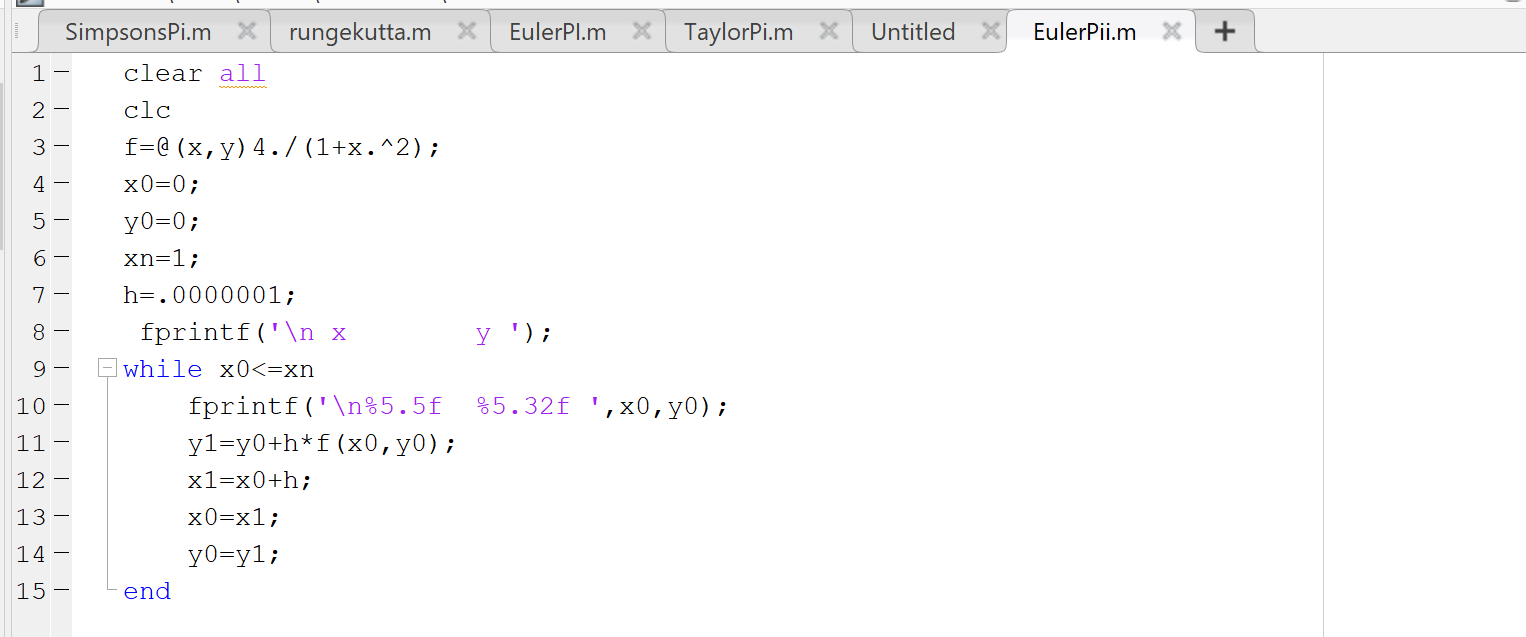
\includegraphics[width=5in, height=2in]{EulerCode.png}
\end{center}
\begin{center}
    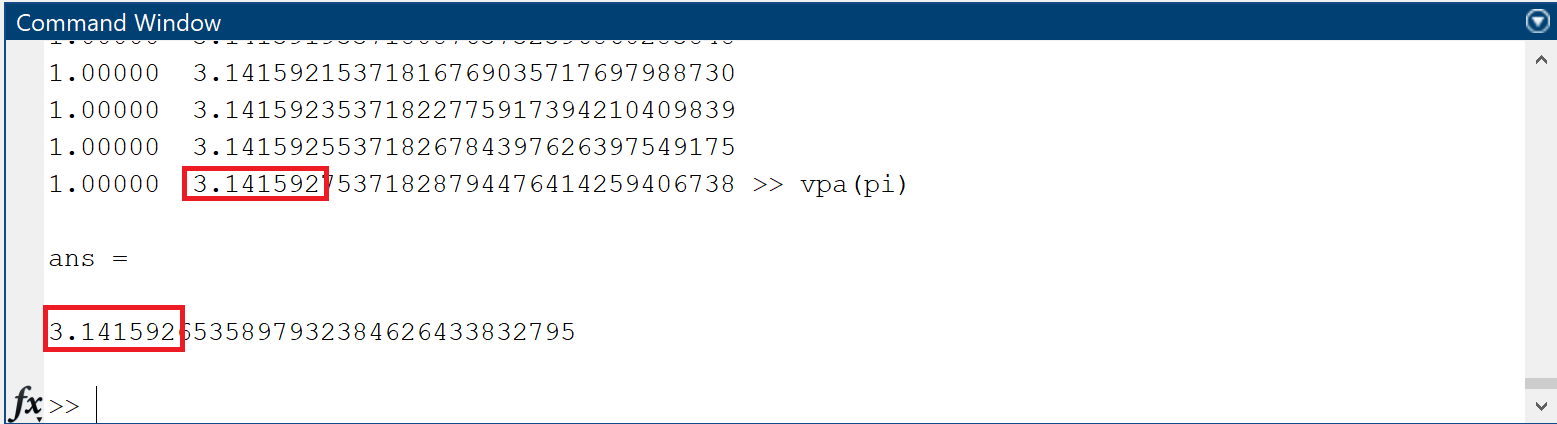
\includegraphics[width=5in, height=2in]{EulerResult.png}
\end{center}
    \item \textbf{Second Order Taylor's Method (Deanna)}
    \\\indent The Higher Order Taylor's method is among one of the standard methods used to compare the accuracy of various numerical methods in order to solve I.V.P or D.E. This method employs the Taylor polynomial of the solution to the equation \cite{Sezer07}. For this particular case, we are working with Taylor's second order polynomial. 
    
    \indent According to Taylor's Theorem, for any solution that uses Taylor expansion at the point $t_{i}$, we have 
    y($t_{i}$+1)= y($t_{i}$)+hy'($t_{i}$)+$\tfrac{h^2}{2}$y''($t_{i}$)+...+
    $\tfrac{h^{n+1}}{(n+1)!}$y^{n+1}$\sigma$ where $\sigma$ is between $t_{i}$ and $t_{i+1}$. The larger the step size, the more accurate the approximation will be using Higher Order Taylor's Method. \cite{Atkinson} Within our given step size, the second order of Taylor's method approximated $\pi$ within 9 digits, which can also be seen in the given Matlab image below. 
    
\begin{center}
    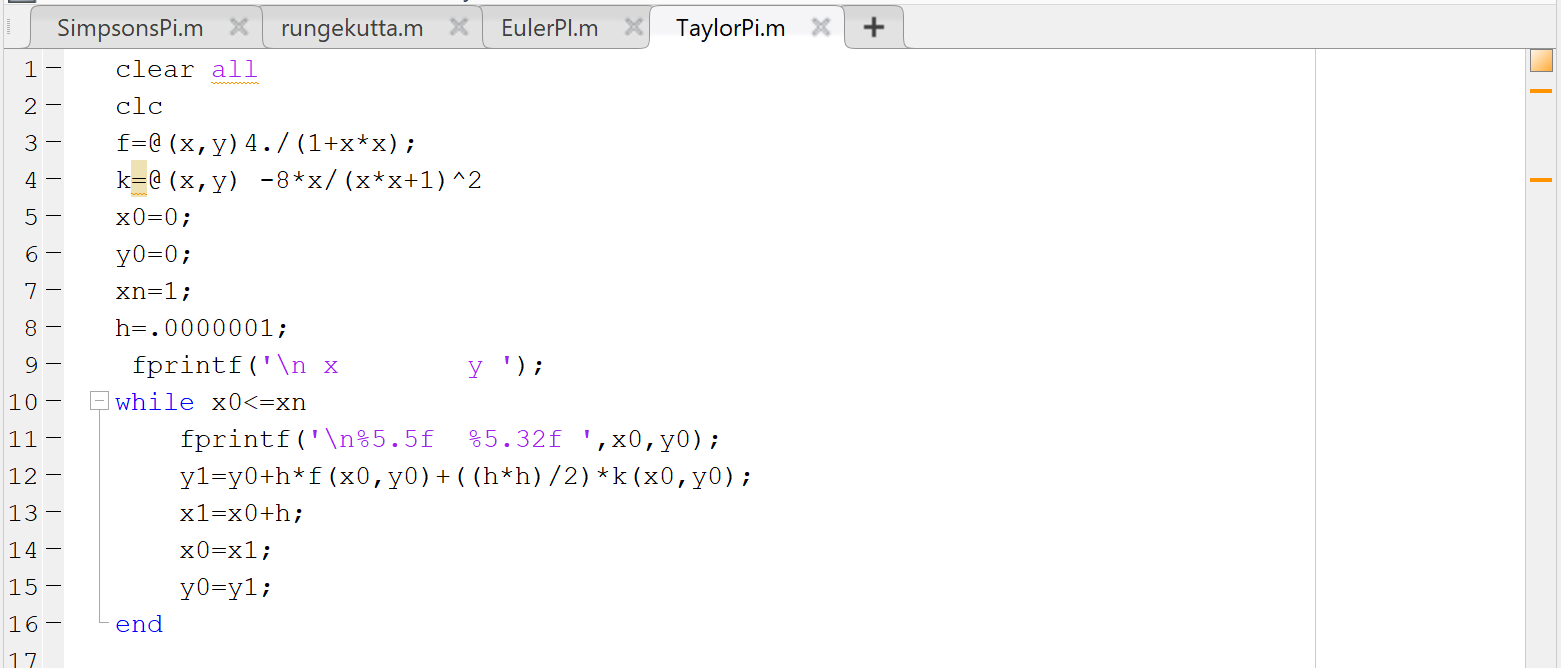
\includegraphics[width=5in, height=2in]{TaylorCode.png}
\end{center}
\begin{center}
    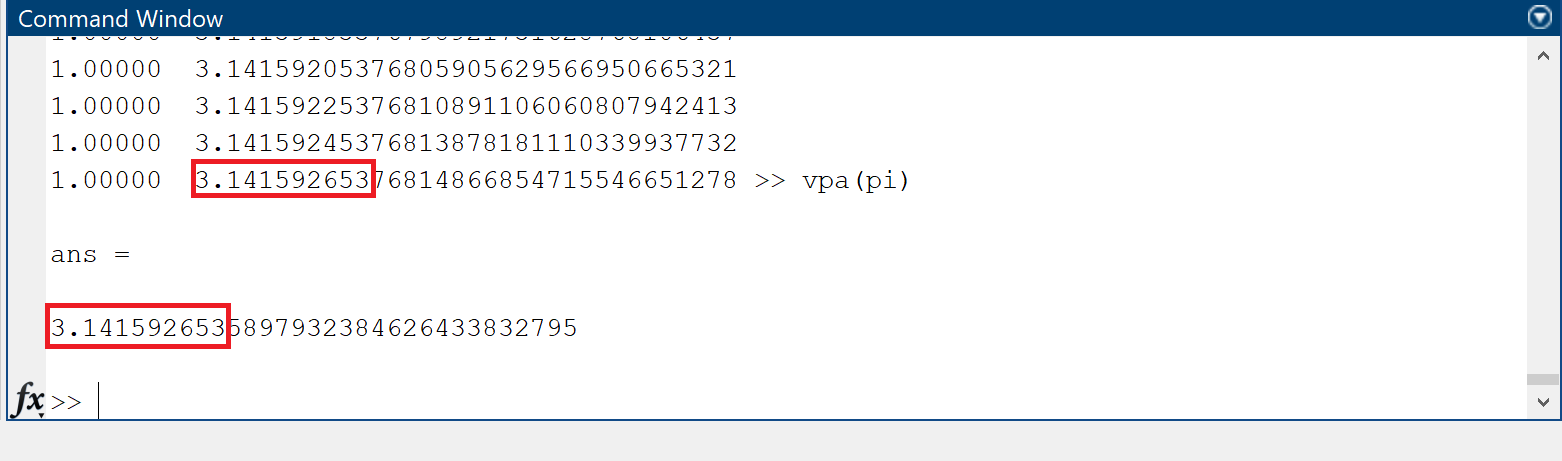
\includegraphics[width=5in, height=2in]{TaylorResult.png}
\end{center}
 
 \indent Using Taylor's method we can calculate the derivative of any Y($t_{i}$) order given and correlate it to it's equivalent Taylor series. \cite{Kiltu17} In the past this has been a major downside of using Taylor's method if you were to calculate the derivative of a very high order approximation by hand. But with the help of programs like Matlab, Taylor's method is now considered an important frame work for Numerical Methods. 
    \item \textbf{Simpson's Rule (Brennon)}
    \\\indent Simpson's Rule is a  numerical integration technique.\cite{Matthews03} Numerical integration is often used when a function has no explicit anti-derivative or if the if the anti-derivative is too difficult to obtain. While this method is generally quite accurate, one disadvantage is that the points must be evenly spaced, or the odd number points must
lie exactly at the midpoint between the even numbered points.\cite{Young18} The technique involves using a sum $ \sum_{i=0}^{n} a_{i}f(x_{i})$ to approximate $\int_{a}^{b} f(x) dx$, where \{$x_{0}...x_{n}$\} is a set of distinct nodes from the interval [a,b]; approximating $\int_{a}^{b} f(x) dx$ is called numerical quadrature.   \cite{Bourne18} Simpson's Rule approximates the value of a definite integral by implementing the use of quadratic functions, specifically it uses parabolas to approximate each piece of the curve. The order of approximation is $O(h^4)$.
    \\\indent Simpson's Rule uses the following equation:
    \begin{center}
    $$ \int_{x_{0}}^{x_{2}} f(x) dx=\tfrac{h}{3}(y_{0}+4y_{1}+y_{2})$$
    \end{center}
\begin{center}
    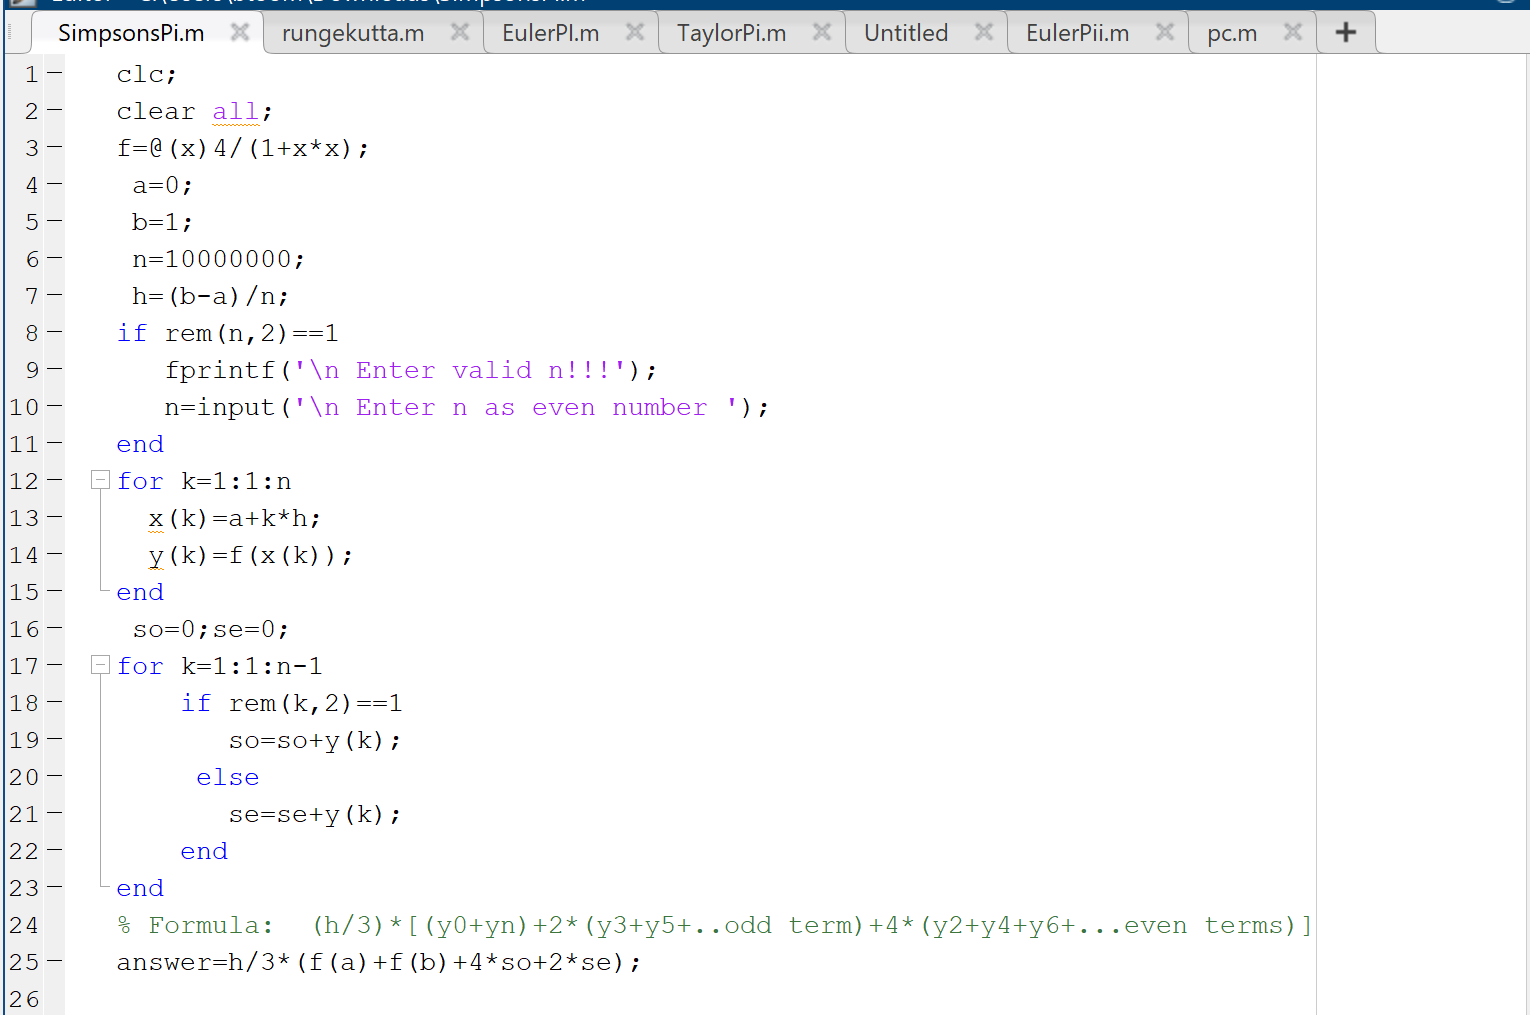
\includegraphics[width=5in, height=3in]{SimpsonsCode.png}
\end{center}
\begin{center}
    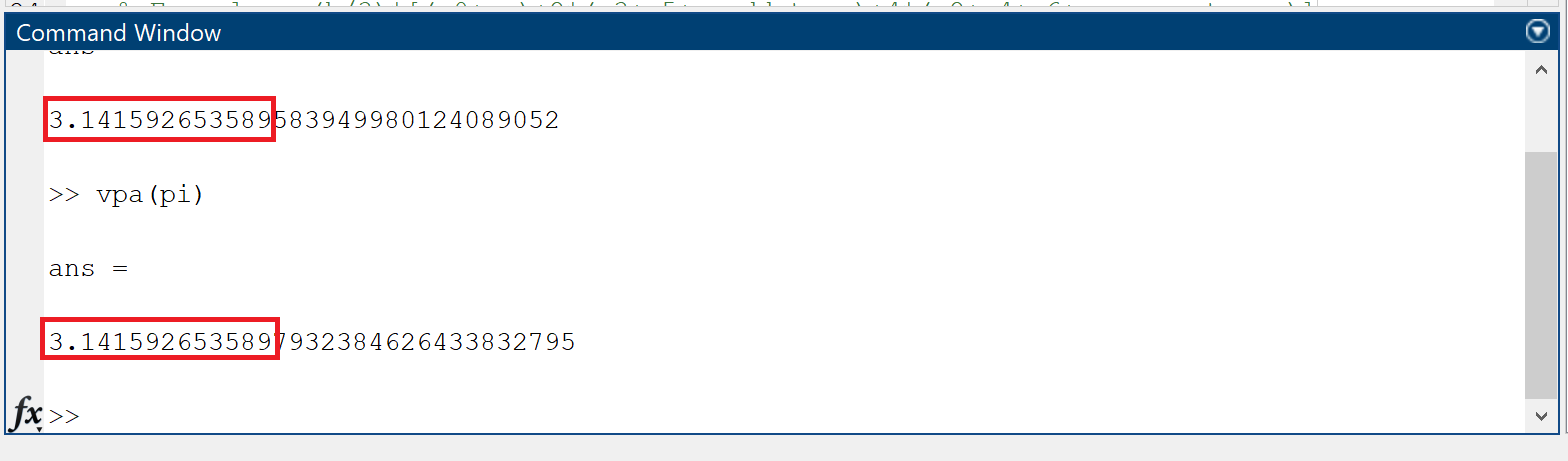
\includegraphics[width=5in, height=2in]{SimpsonResult.png}
\end{center}
Simpson's Rule is able to approximate $\pi$ to twelve decimal places.
    \item \textbf{Fourth Order Runge-Kutta Method (Alexa)}
    \\ \indent Runge-Kutta methods, like Taylor methods, have a high-order local truncation error. However, unlike Taylor, it excludes the calculations of higher order derivatives of $f(t,y)$ and thus, it's less time consuming and more efficient.\cite{Burden15} This method iterates the x-values, increasing a fixed step size of h at each iteration. \cite{Barker17} 
    \\\indent In this case, we are looking at the Fourth Order Runge-Kutta method, which is the most commonly used as it gives more accurate answers. This uses four approximations per step size. The local truncation error of the fourth order is $O(h^4)$ where as the local truncation error for higher-order methods is $O(h^{n-1})$ and thus, explains why methods of order less than five, with smaller step sizes, are used in preference. 
    \\\indent The Fourth Order Runge-Kutta method formula is the following:
    \begin{center}
    \\$y_{i+1}=y_{i}+\tfrac{1}{6}(k_{1}+2k_{2}+2k_{3}+k_{4})$
    \\$k_{1}=hf(t_{i},y_{i})$
    \\$k_{2}=hf(t_{i}+\tfrac{h}{2},y_{i}+\tfrac{1}{2}k_{1})$
    \\$k_{3}=hf(t_{i}+\tfrac{h}{2},y_{i}+\tfrac{1}{2}k_{2})$
    \\$k_{4}=hf(t_{i+1},y_{i}+k_{3})$
    \\ for each $i=0,1,...,N-1$
    \end{center}
\begin{center}
    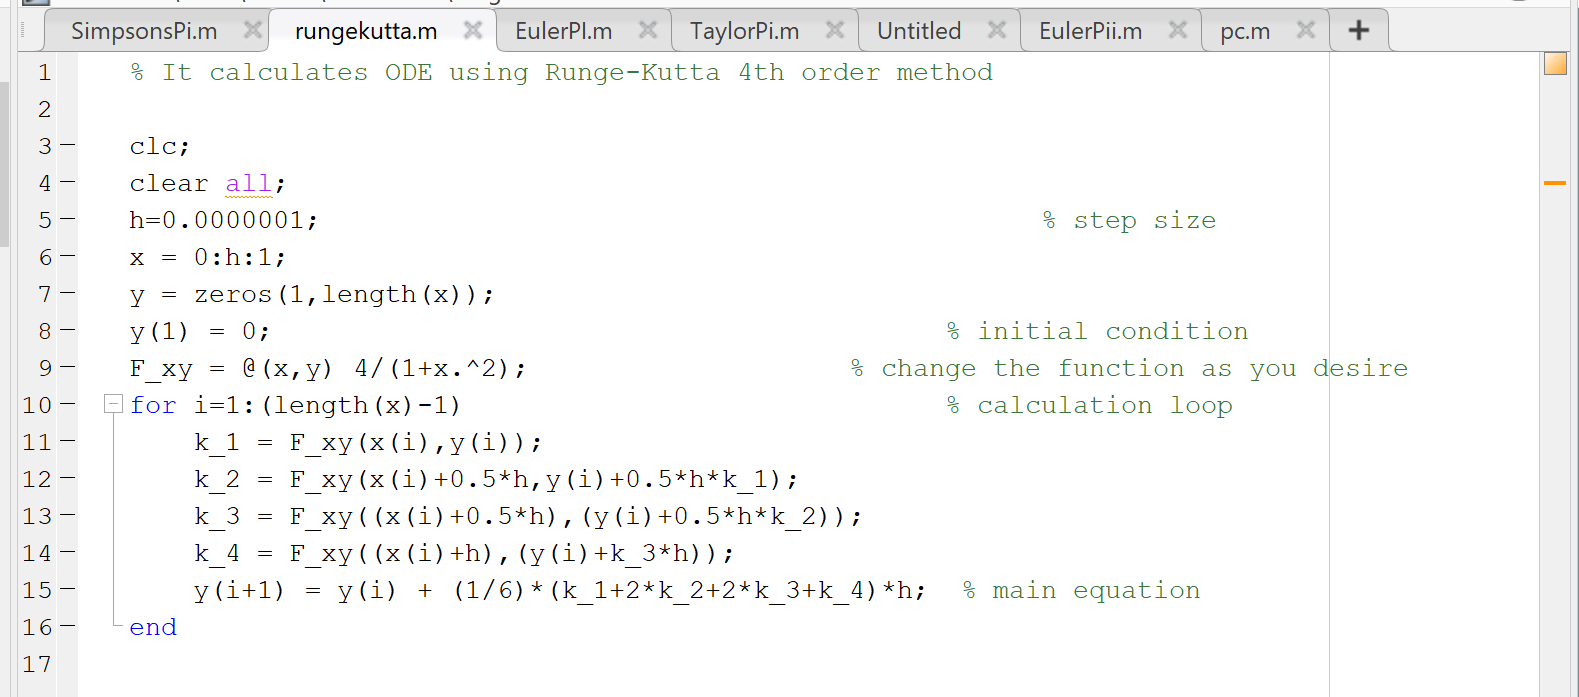
\includegraphics[width=5in, height=2in]{RungeKCode.png}
\end{center}
\begin{center}
    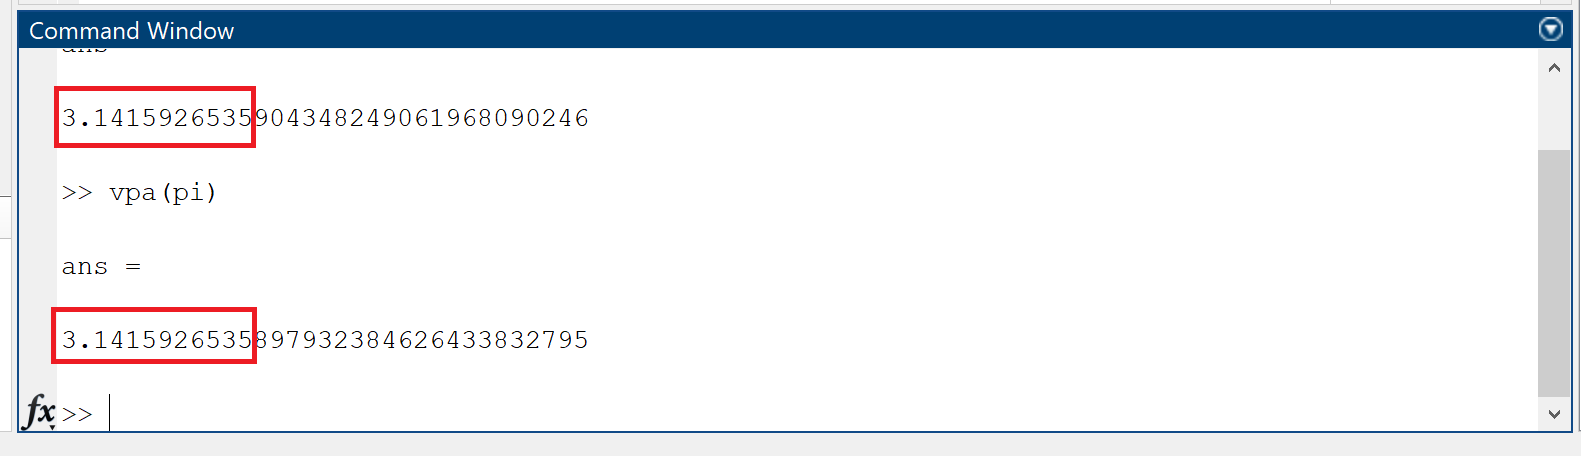
\includegraphics[width=5in, height=2in]{RungeKResult.png}
\end{center}
\\
\indent Based on the results above, Fourth Order Runge-Kutta approximates $\pi$ up to ten decimal places.
    \item \textbf{Adams Fourth Order Predictor-Corrector Method (Kenya)}
    \\ \indent The Adams-Bashforth and Adams-Moulton techniques are multi-step methods, which means each approximation at a mesh point $t_{k+1}$ relies on various approximations at mesh points $t_{k+1}$ to $t_{k}$. This is dissimilar to previous methods used such as Euler’s Method and Runge-Kutta method which are one-step methods, i.e. they rely only on the immediately preceding approximation to calculate future approximations \cite{Burden15}
    
    The Adams fourth-order predictor-corrector method uses fourth-order Adams-Bashforth as the predictor and fourth-order Adams-Moulton as the corrector. A predictor-corrector method uses an explicit method to predict and implicit method to correct or improve the approximation. 
    By using these methods together, the formula becomes: 
    \begin{center}$P_{n+1}=y_{n} + \frac{h}{24}(55f(t_{n},y_{n})-59f(t_{n-1},y_{n-1})+37f(t_{n-2},y_{n-2})-9f(t_{n-3},y_{n-3}))$
    \\$y_{n+1}=y_{n}+\frac{h}{24}(9f(t_{n+1},P_{n+1})+19f(t_{n},y_{n})-5f(t_{n-1},y_{n-1})+f(t_{n-2},y_{n-2}))$ \cite{Burden15}
    \end{center}

    The fourth-order Adams-Bashforth method needs four previous approximations, thus we used Runge-Kutta to approximate these previous points. 
\\
\begin{center}
    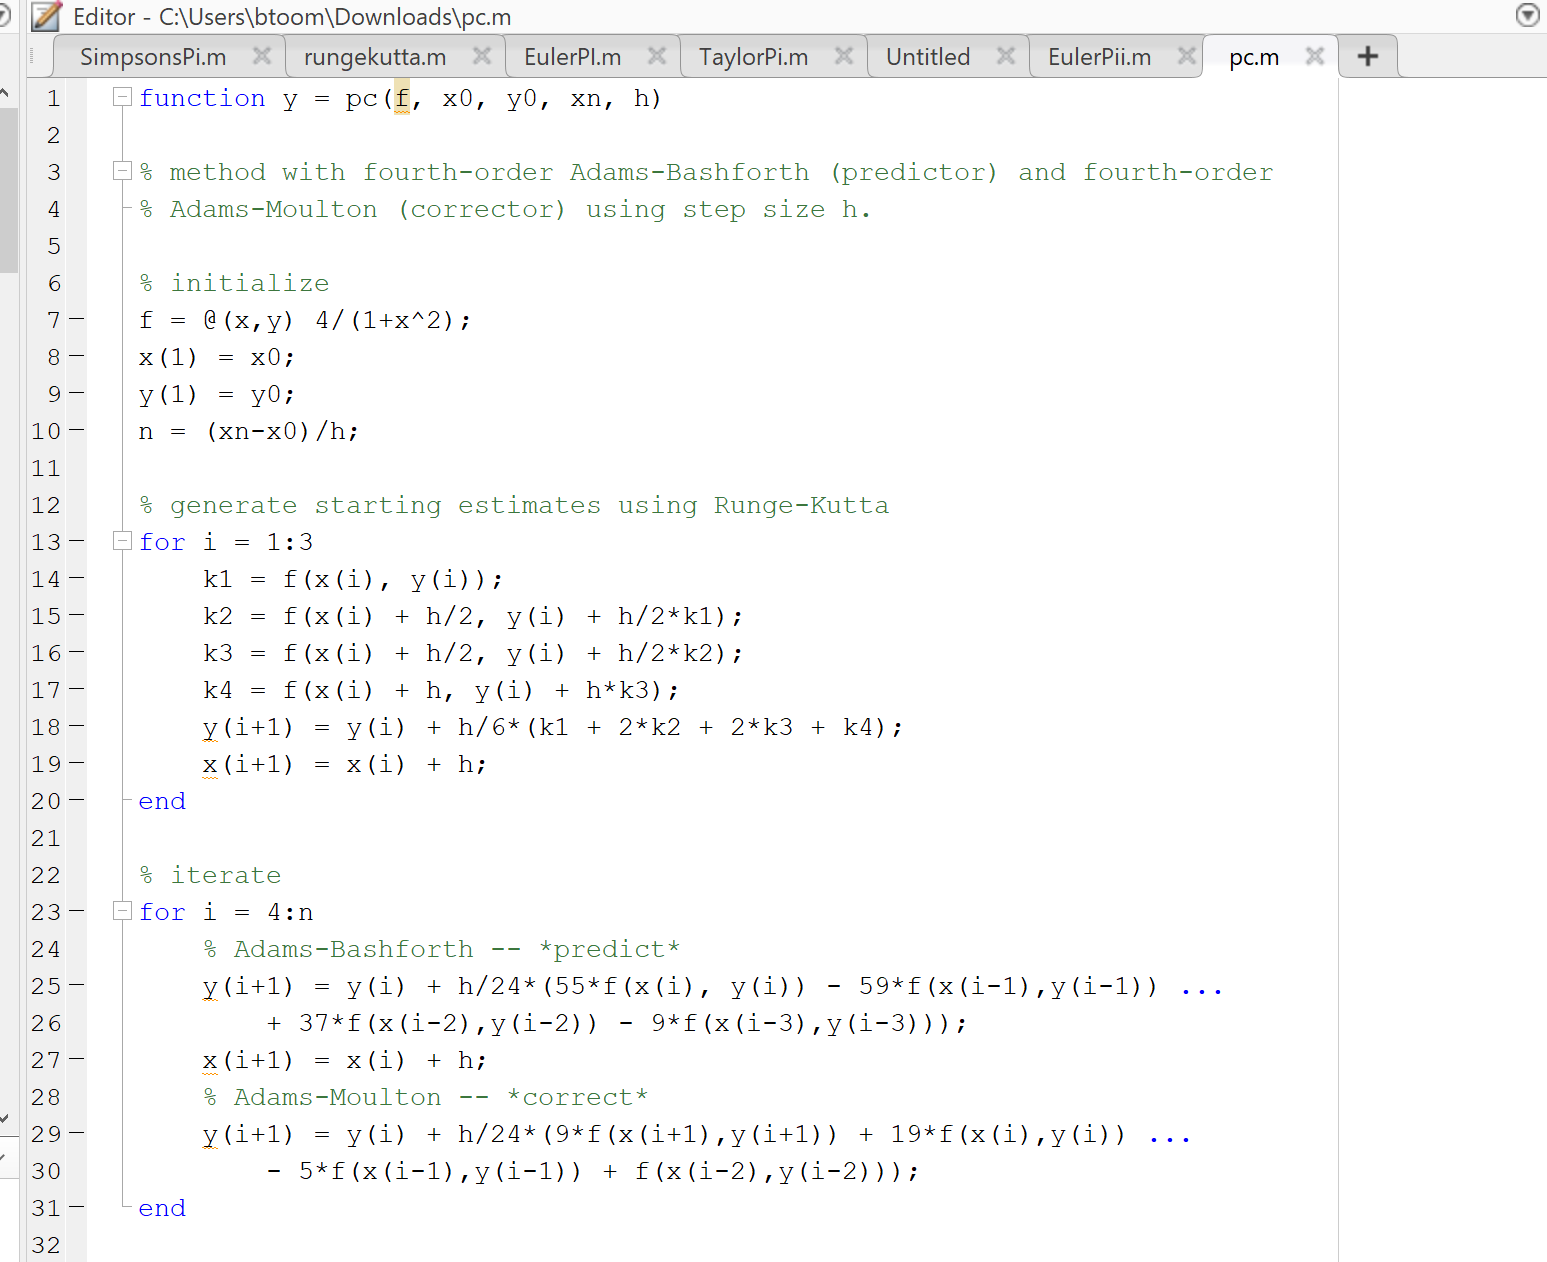
\includegraphics[width=5in, height=3in]{AdamsCode.png}
\end{center}
\begin{center} 
    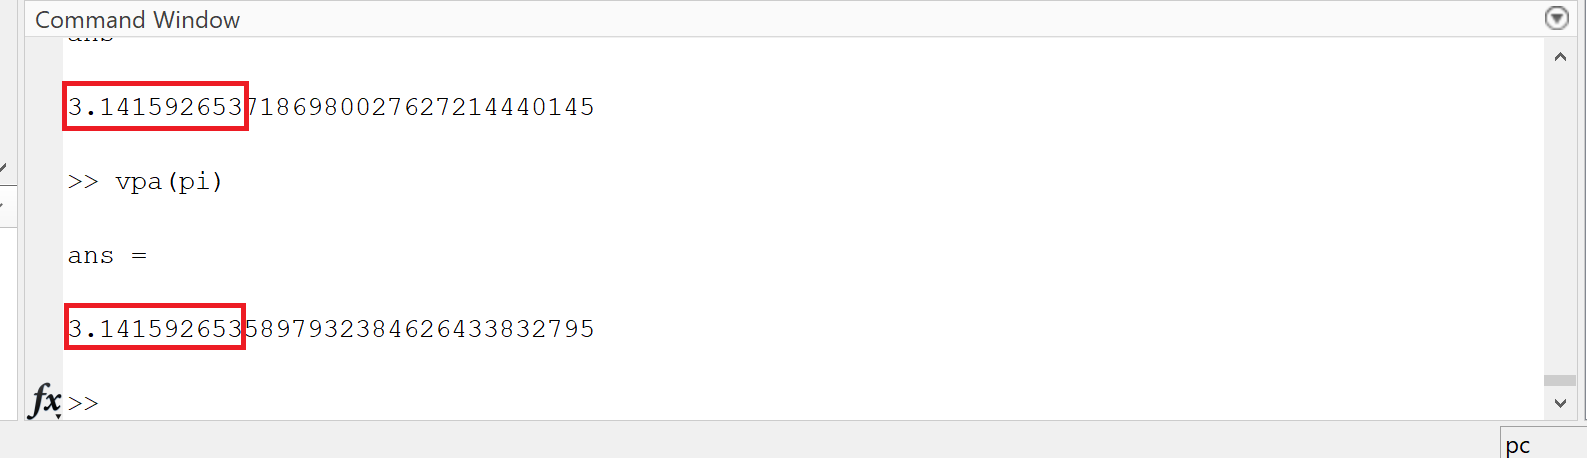
\includegraphics[width=5in, height=1.5in]{AdamsResult.png}
\end{center} \cite{Dobrushkin}
\\ 
\indent As seen in the result above, this method approximates $\pi$ accurately up to 9 decimal places, which is a sufficient approximation of $\pi$ for most usages in general calculations. 
\section{Conclusion}

\indent As seen from the results above, Euler's method was the least accurate of the methods shown, estimating $\pi$ to only six decimal places. Adams and Taylor's method approximated $\pi$ within nine decimal places, while Runge-Kutta was the second most accurate, approximating $\pi$ to ten decimal places. This leaves Simpson's method as our most accurate approximation, correctly approximating $\pi$ up to twelve decimal places. This is possibly due to the fact that the equation used for $\pi$ is an integral itself, thus making numerical integration more accurate than approximating the exact solution to the integral explicitly. In addition to this, Simpson's Rule takes into account parabolas to approximate each part of the curve. This gives a more accurate and more efficient approximation than the other numerical integration methods. 

\pagebreak

\begin{thebibliography}{9}
\bibitem{Atkinson}
  Atkinson, Kendall E.,
  \textit{Taylor Series Method},
  University of Iowa,
  2007.
\bibitem{Barker17}
  Barker, Christopher A.,
  \textit{Numerical Methods for Solving Differential Equations},
  Mathematics and Science Learning Center, San Joaquin Delta College,
  2017.
\bibitem{Burden15}
  Burden, Faires, Burden,
  \textit{Numerical Analysis},
  Cenagage Learning, 
  2015.
\bibitem{Bourne18}
  Bourne, Murray,
  \textit{Simpson's Rule},
  Interactive Mathematics, 
  2018.
\bibitem{Crowl01}
  Crowl, Lindsay
  \textit{Investigating Euler’s Method and Differential Equations to Approximate $\pi$},
  University of Utah, 
  2001.
\bibitem{Dobrushkin}
  Dobrushkin, Vladimir,
  \textit{Adams fourth-order predictor-corrector MATLAB code},
  Brown University.
\bibitem{Gorleau03}
  Gorleau, Rick,
  \textit{Approximating Pi},
  PBS, Public Broadcasting Service,
  2003.
\bibitem{Kaw09}
  Kaw, Kalu,
  \textit{Numerical Methods With Applications},
  University of South Florida, 
  2009.
\bibitem{Kiltu17}
  Kiltu, Gashu & Garoma, Habtamu,
  \textit{Comparison of Higher Order Taylor's Method and Runge- Kutta Methods for Solving First Order Ordinary Differential Equations},
  Journal of Computer and Mathematical Sciences,
  2017.
\bibitem{Lamb12}
  Lamb, Evelyn,
  \textit{How Much Pi Do You Need?},
  Scientific American Blog Network, Scientific American,
  2012.
\bibitem{Matthews03}
  Matthews, John H.,
  \textit{Module for Simpson's Rule for Numerical Integration},
  California State University Fullerton,
  2003.
\bibitem{Sezer07}
  Mehmet,Dascioglu,
  \textit{A Taylor method for numerical solution of generalized panto-graph equations with linear functional argument},
  Journal of Computational and Applied Mathematics, Science Direct,
  2007.
  \bibitem{Young18}
  Young, Mohlenkamp
  \textit{Lecture 22
Integration: Midpoint and Simpson’s Rules
},
  Ohio University,
  2018.
\end{thebibliography}


\end{document}
